\section{端到端评估}
\label{sec:eval}

\noindent
在对高效 LLM 调度的研究收尾时，我们通过端到端 LLM 服务性能，比较 {\sys} 的乘法方法（见 \textsection{\ref{sec:method}}）与当前最先进的调度器。

\begin{figure}[!t]
    \centering
    \begin{subfigure}{\linewidth}
        \centering
        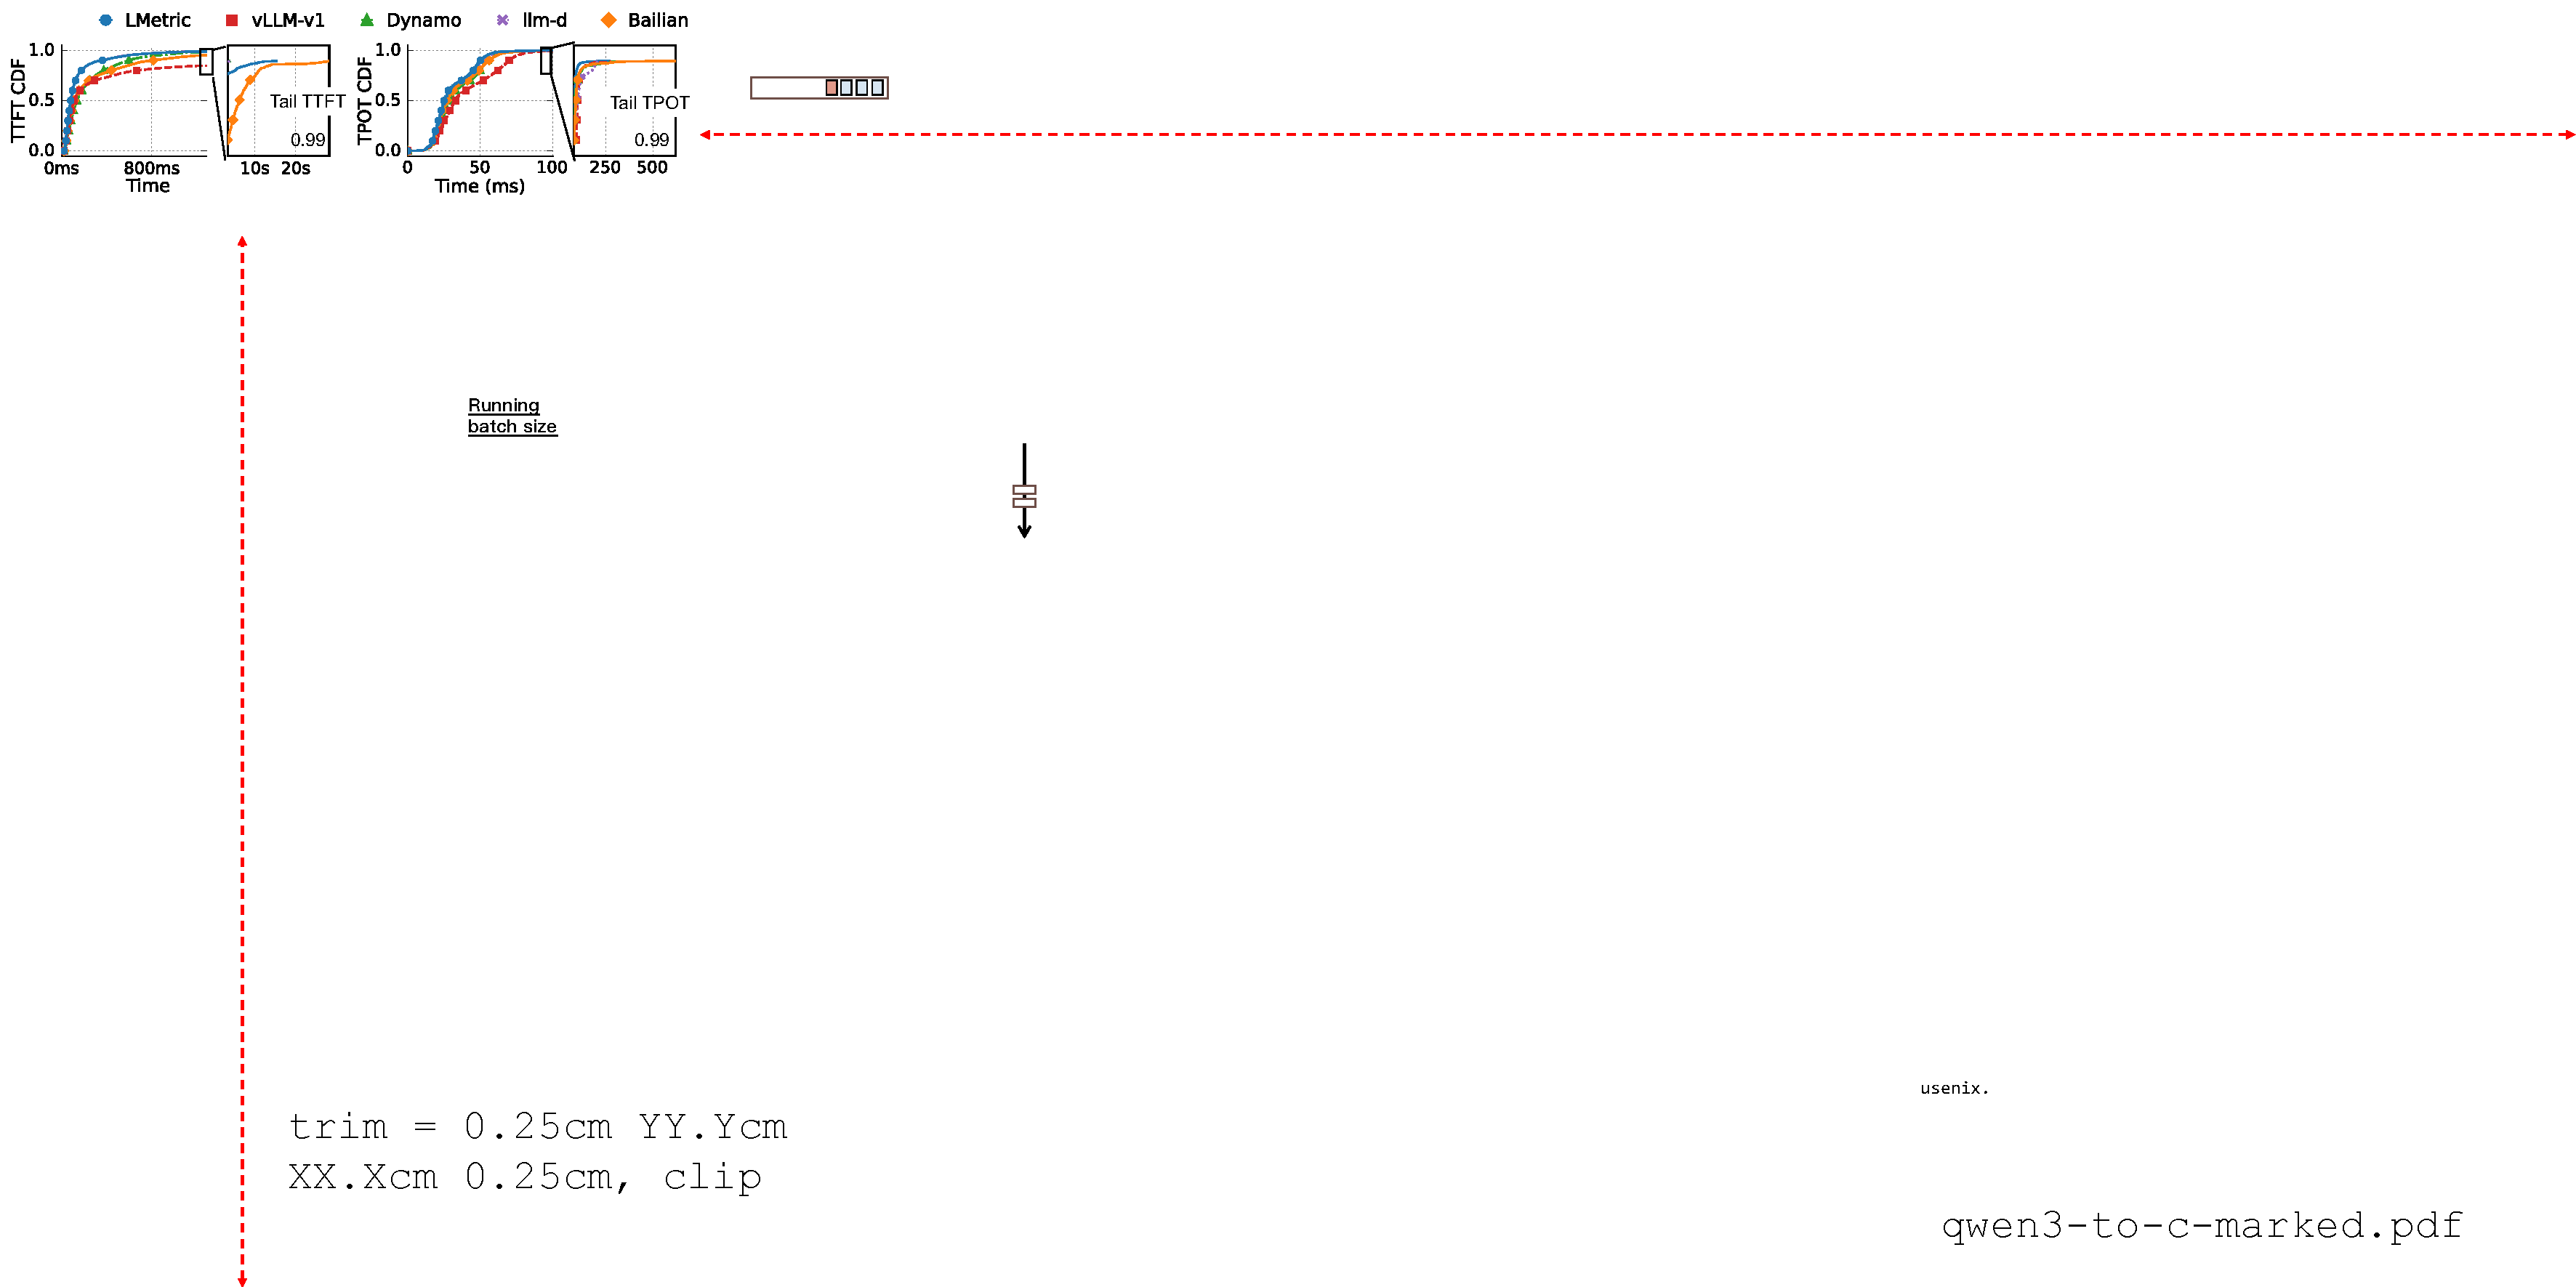
\includegraphics[width=0.98\linewidth, trim=0.25cm 25.2cm 43.75cm 0.25cm, clip]{figs/e2e-cdf-v1/qwen3-to-c-marked.pdf}
        \vspace{-8pt}
        \caption{\small{Qwen3-30B 在 ChatBot (Qwen) 工作负载上。}}
        \label{fig:eval-qwen3-to-c}
    \end{subfigure} \\[6pt]
    \begin{subfigure}{\linewidth}
        \centering
        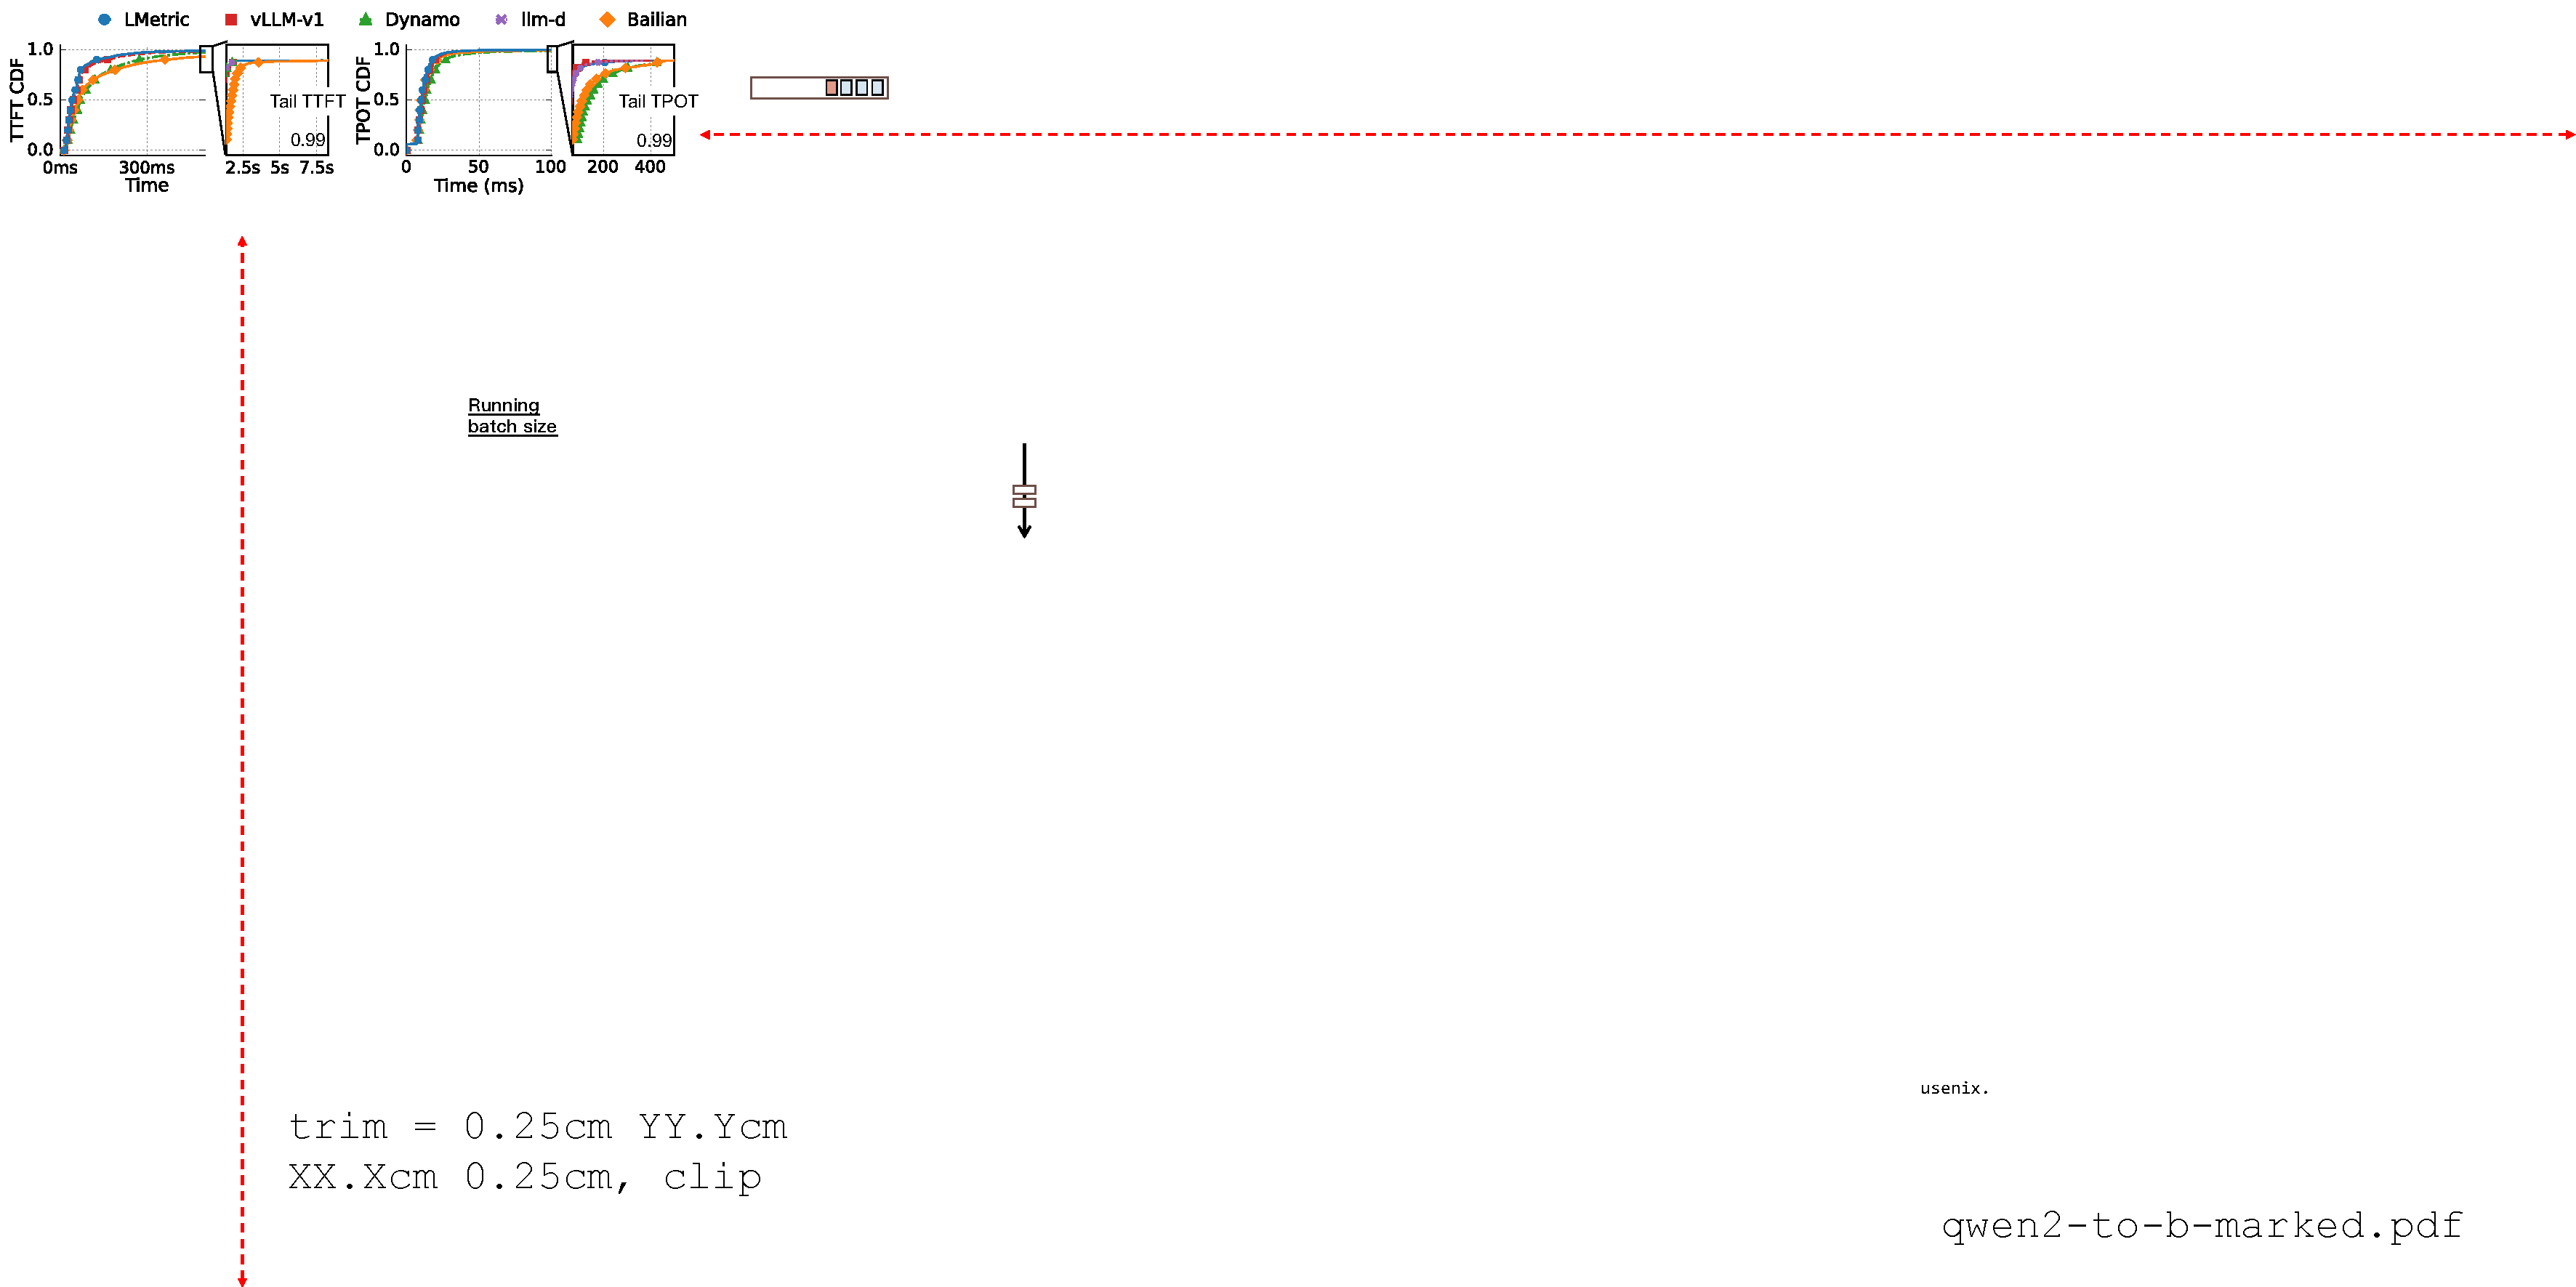
\includegraphics[width=0.98\linewidth, trim=0.25cm 25.2cm 43.75cm 0.25cm, clip]{figs/e2e-cdf-v1/qwen2-to-b-marked.pdf}
        \vspace{-8pt}
        \caption{\small{Qwen2-7B 在 Agent (Qwen) 工作负载上。}}
        \label{fig:eval-qwen2-to-b}
    \end{subfigure} \\[6pt]
    \begin{subfigure}{\linewidth}
        \centering
        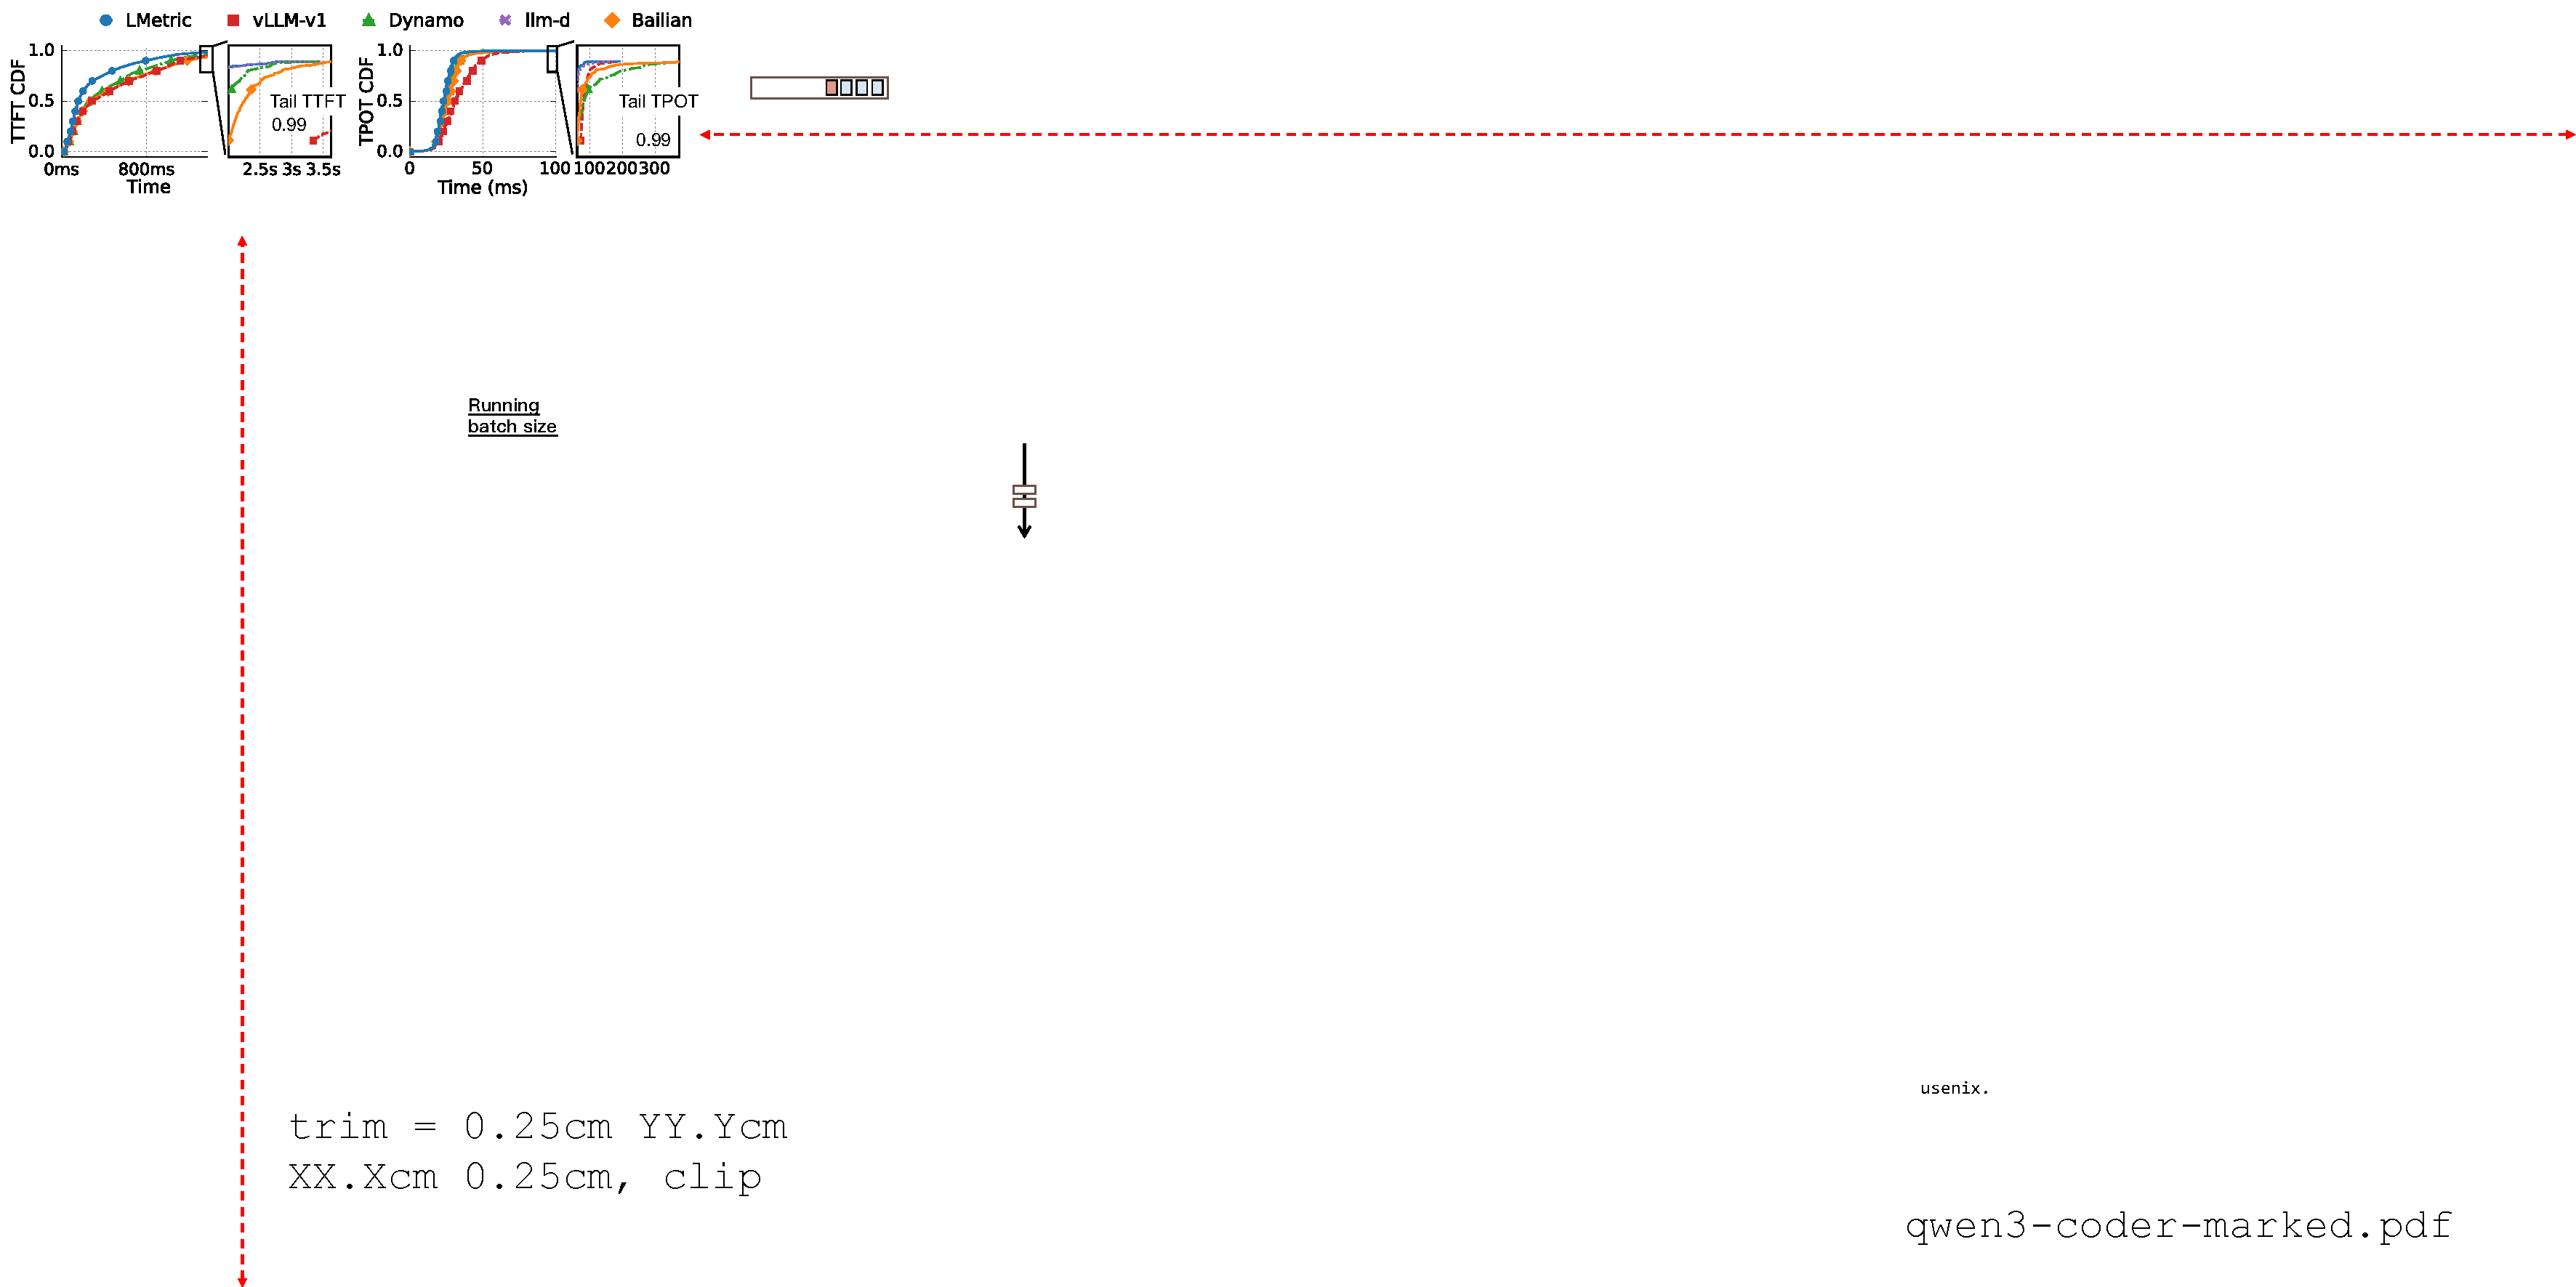
\includegraphics[width=0.98\linewidth, trim=0.25cm 25.2cm 43.75cm 0.25cm, clip]{figs/e2e-cdf-v1/qwen3-coder-marked.pdf}
        \vspace{-8pt}
        \caption{\small{Qwen3-30B 在 Coder 工作负载上。}}
        \label{fig:eval-qwen3-coder}
    \end{subfigure} \\[6pt]
    \begin{subfigure}{\linewidth}
        \centering
        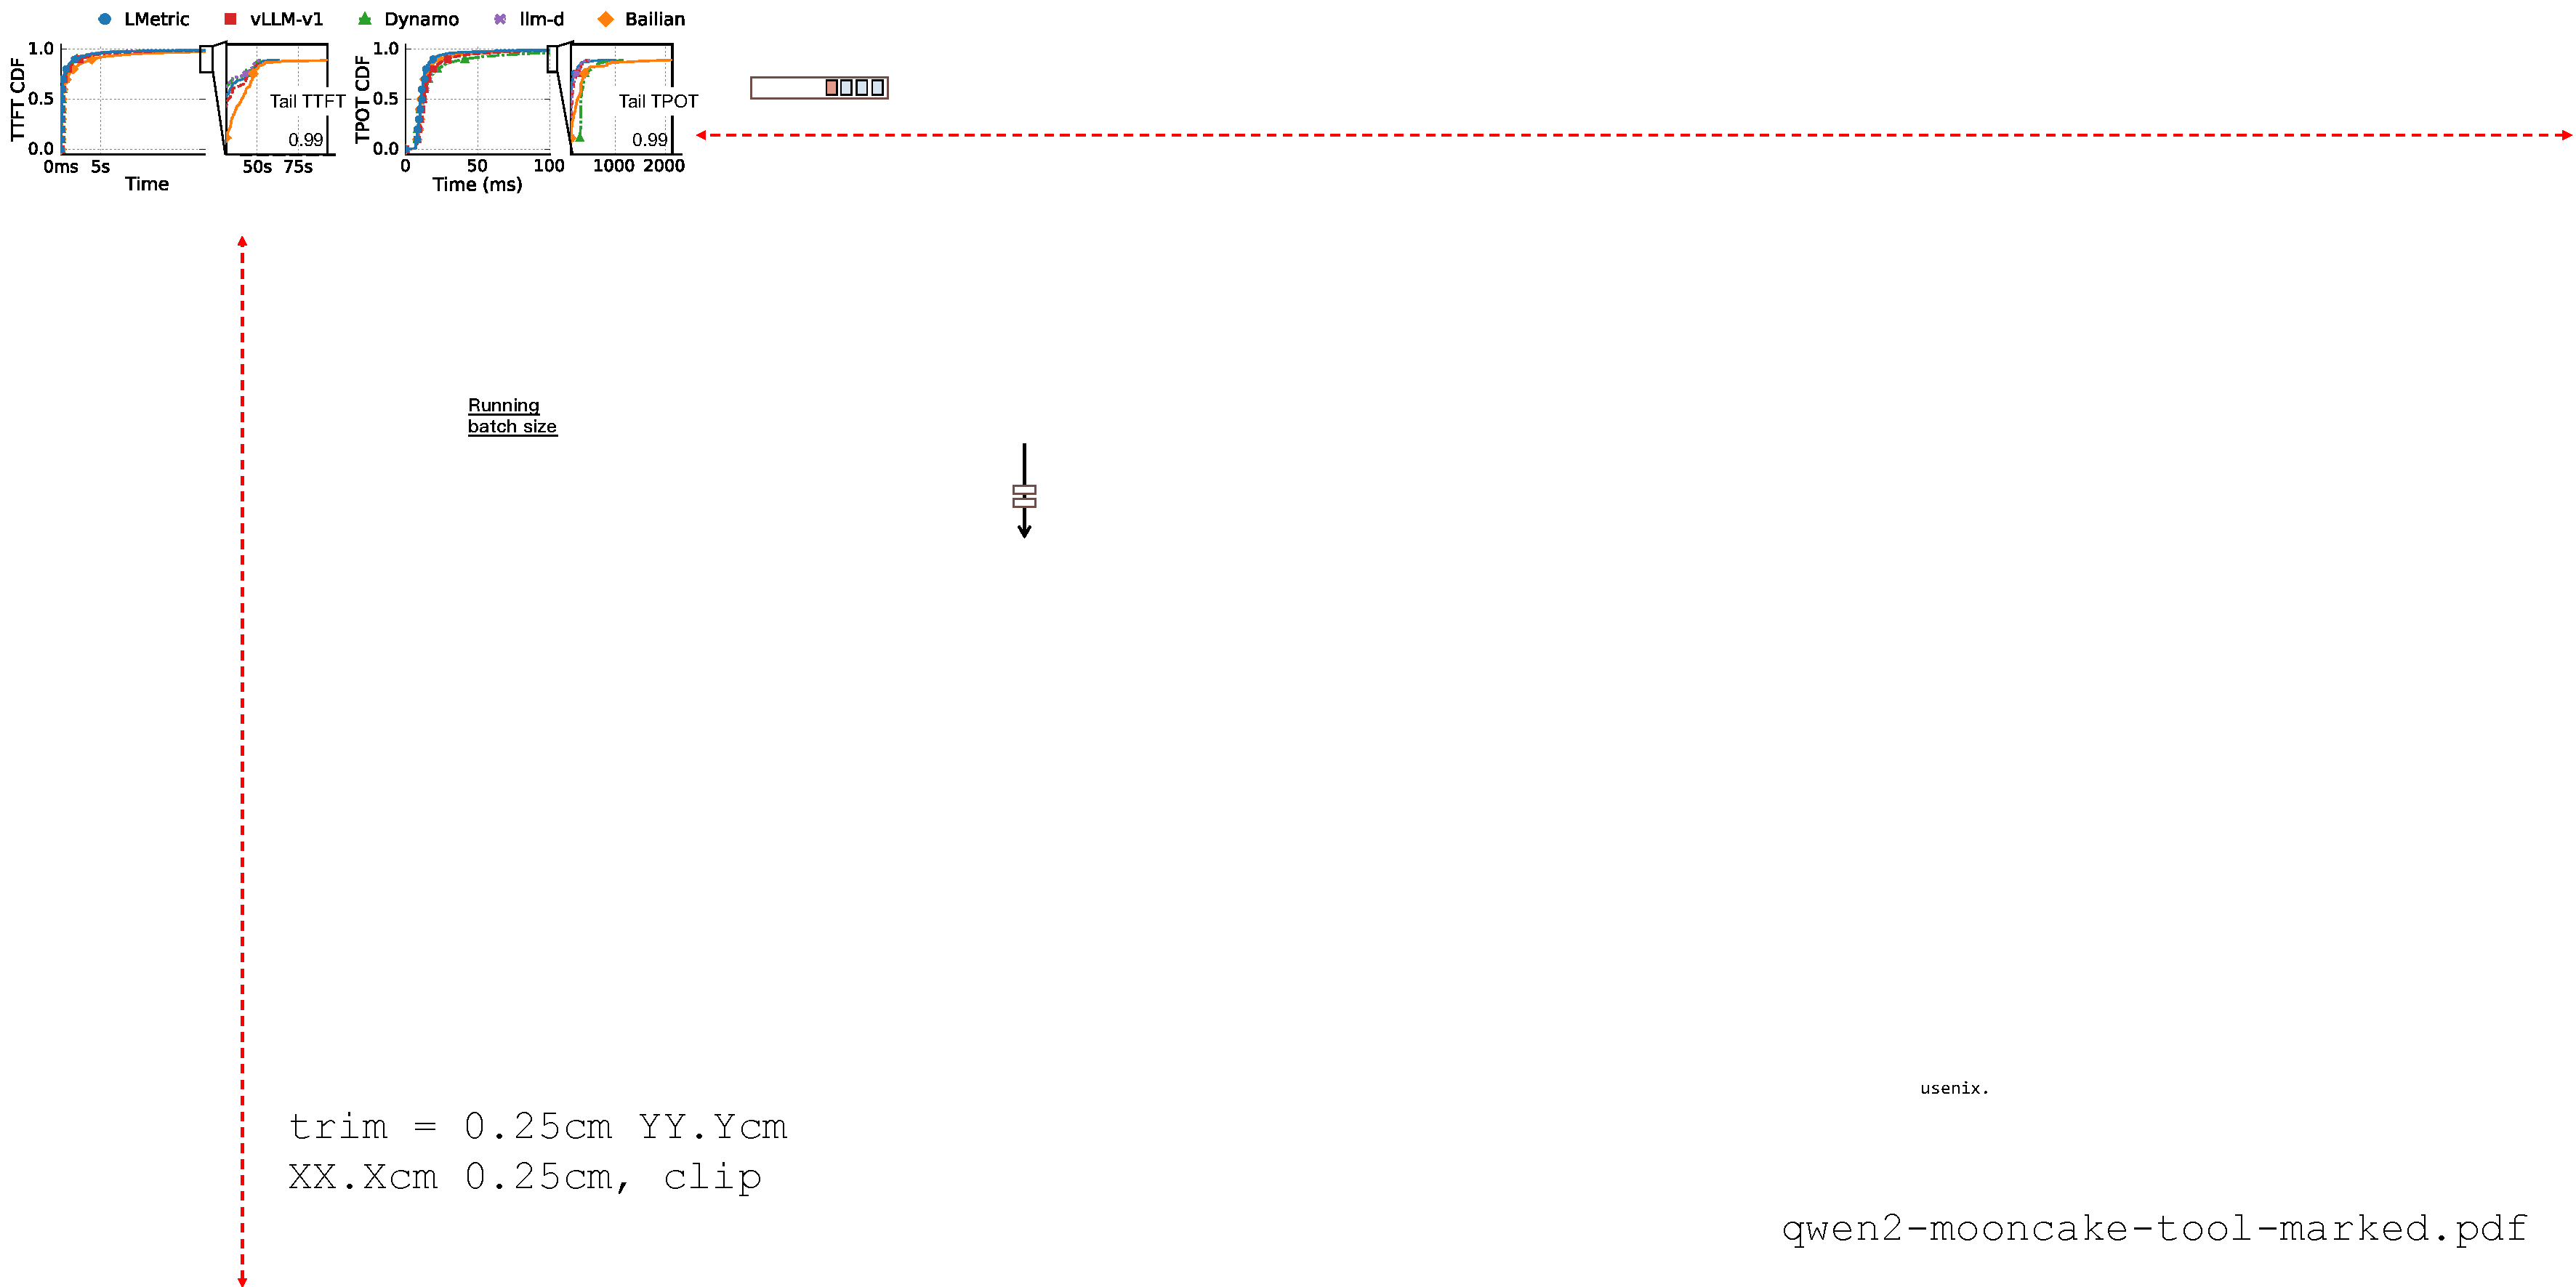
\includegraphics[width=0.98\linewidth, trim=0.25cm 25.2cm 43.75cm 0.25cm, clip]{figs/e2e-cdf-v1/qwen2-mooncake-tool-marked.pdf}
        \vspace{-8pt}
        \caption{\small{Qwen3-30B 在 Agent (Kimi) 工作负载上。}}
        \label{fig:eval-qwen2-mooncake-tool}
    \end{subfigure}
    \caption{\small{{\sys} 与各基线在四个工作负载上的端到端 TTFT 与 TPOT CDF。}}
    \label{fig:eval-cdf}
\end{figure}

\begin{figure*}[!t]
    \centering
    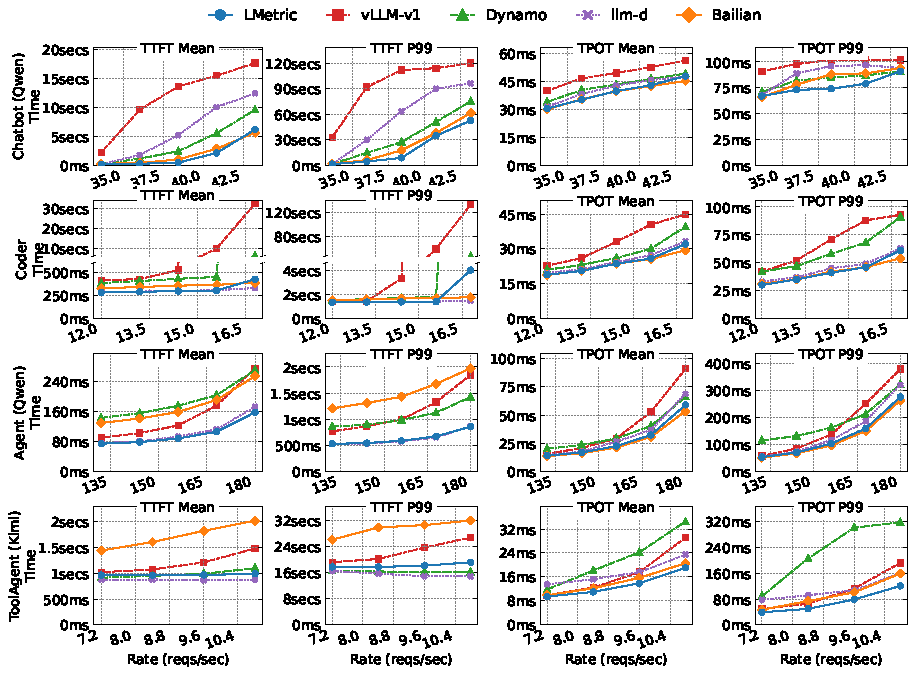
\includegraphics[width=0.9\linewidth]{./figs/scaling-test/scaling-fix-v1.pdf} \\[-3pt]
    \caption{\small{%
    不同请求速率下的端到端性能。
    除第二行使用 Qwen2-7B 模型外，其余各行均使用 Qwen3-30B 模型。
        }}
    \label{fig:scaling-test}
\end{figure*}

\stitle{基线方法。\,}
我们将 {\sys} 与开源调度器以及 {\company} 当前生产环境所使用的调度器进行比较。
由于一些实现会因为路由器本身的问题表现不佳，
例如 vLLM 的 Python 路由器就存在吞吐偏低的问题~\cite{vllm-bug}，
我们将这些策略重新实现在 \textsection{\ref{sec:factory}} 所述的高性能 Rust 路由框架中。
为了做到真正可比的横向比较，
我们在统一框架下比较这些策略，
并仔细验证了我们的重实现不会慢于原始实现。
各基线的详细说明如下：
\\[-15pt]
\begin{itemize}[leftmargin=*,leftmargin=10pt,itemindent=0pt]
\item \textbf{{\company}} 是 {\company} 的 LLM 服务系统中正在使用的生产级调度器。
    它采用了一种与 {\fig{fig:vllm-kvcache}} (b) 所示类似的线性组合方法。
    我们针对每个工作负载都仔细调节了其超参数，以获得最佳性能。
     \\[-15pt]

\item \textbf{vLLM~\cite{vllm-code}} 是一个被广泛使用的 LLM 服务系统，
    采用 {\fig{fig:vllm-kvcache}} (a) 所描述的“仅负载均衡”设计。
    
\item \textbf{Dynamo~\cite{ai-Dynamo}} 是 NVIDIA 发布的流行服务框架。
    它同样采用基于线性组合的方式，但所选指标与 {\company} 不同。
    其用于 {\kvcache} 感知的指标是预填充 token 数（与我们的 P-token 相同），
    用于负载均衡的指标则是实例上的总 token 数。
    路由器会将请求发送到这两个指标经归一化并加权求和后最小的实例。
    与 {\company} 类似，我们也为其在每个工作负载上调节超参数，以获得最优性能。 \\[-15pt]

    \item \textbf{llm-d~\cite{llm-d}} 采用基于时延的调度策略：
    它会估计 TTFT，并依据 \textsection{\ref{sec:prediction-combination}} 所述的模拟方法，把请求路由到估计 TTFT 最低的实例。 \\[-15pt]
\end{itemize}


\stitle{整体性能。\,}
{\fig{fig:eval-cdf}} 展示了 {\sys} 与其他基线在四条轨迹上的端到端 TTFT 与 TPOT CDF。
所有实验都在一套 16 GPU、16 实例的测试床上进行，
并将轨迹缩放到测试床可承载最大负载的一半。
由于篇幅限制，我们只报告具有代表性的结果子集：
Qwen3 MoE 模型在 ChatBot、Coder 和 Agent 工作负载上的结果，
以及 Qwen2 模型在 API 工作负载上的结果。
我们观察到，在所有“模型—轨迹”组合上，性能趋势都保持一致。

{\sys} 在所有轨迹上都优于全部基线。
在 ChatBot 工作负载上，
与 vLLM 相比，它将平均 TTFT 降低了 92\%，将平均 TPOT 降低了 24\%；
与 llm-d——第二好的策略——相比，它在 TTFT 近似的情况下，将 P99 TPOT 降低了 13\%。
性能提升的主要原因在于：它具备 {\kvcache} 感知能力，同时又没有牺牲负载均衡。
为了进一步理解 {\sys} 的行为，
{\fig{fig:eval-e2e-kvcache}} 绘制了在 ChatBot 工作负载上，不同系统的 {\kvcache} 命中率。
可以看到，{\sys} 始终能够获得与其他 {\kvcache} 感知策略相当的 {\kvcache} 命中率，
并且显著高于不感知 {\kvcache} 的策略（vLLM）。
与此同时，
{\fig{fig:eval-e2e-imbalance}} 进一步沿用 \textsection{\ref{sec:challenge-balancing}} 的分析方法，对负载失衡进行了剖析。
为了便于展示，我们只比较 {\sys} 与 llm-d——后者是在 ChatBot 轨迹上表现第二好的方法。
可以看到，相比 llm-d，{\sys} 实现了更均衡的负载。

\begin{figure}[!t]
    \centering
    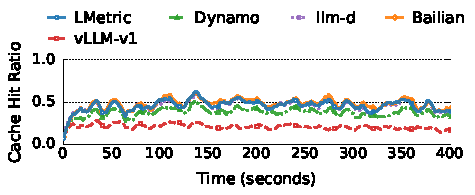
\includegraphics[width=0.98\linewidth]{figs/e2e-kvcache-hit/e2e-kv2.pdf} \\[-0pt]
    \begin{minipage}{1\linewidth}
    \caption{\small{   
        Qwen3-30B 模型在 ChatBot (Qwen) 工作负载上，各策略的 KVCache 命中率对比。
    }}
    \label{fig:eval-e2e-kvcache}
    \end{minipage} \\[-5pt]
\end{figure} 


\begin{figure}[!t]
    \centering
    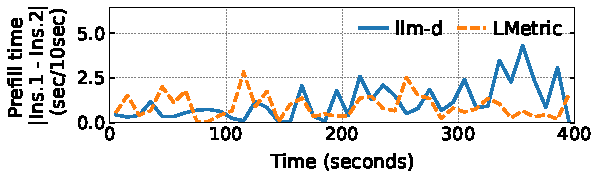
\includegraphics[width=0.98\linewidth]{figs/e2e-kvcache-hit/e2e-lmd-v1.pdf} \\[0pt]
    \begin{minipage}{1\linewidth}
    \caption{\small{   
        {\sys} 与 llm-d 在服务 ChatBot (Qwen) 工作负载、使用 Qwen3-30B 模型时，
        两台实例之间工作负载失衡情况的剖面图。
        图中报告的指标是每个 10 秒时间窗内，两台实例（Inst.）已服务预填充时间的绝对差值。
    }}
    \label{fig:eval-e2e-imbalance}
    \end{minipage} \\[-5pt]
\end{figure} 

\stitle{不同请求速率下的性能。\,}
{\fig{fig:scaling-test}} 进一步展示了 {\sys} 在不同请求到达率下的表现。
结果与固定请求速率设置下基本一致：
在不同轨迹和请求速率上，{\sys} 都优于其他基线；
唯一的例外是 ToolAgent 轨迹，
在该轨迹上，{\sys} 的平均 TTFT 比 llm-d 略高（10\%），
但 TPOT 降低了 30\%。
这可能是因为基于模拟的方法能够比我们简单的 P-token 指标更好地估计预填充工作量。
尽管如此，{\sys} 依然在不依赖复杂模拟器的前提下取得了最低的 TPOT，
因为它同时考虑了 {\kvcache} 管理与（解码）负载均衡。
随着请求速率提高，不同基线之间的性能差距会进一步拉大，
因为在高负载下，更均衡且更具 {\kvcache} 感知能力的调度策略能够更有效地提升系统整体吞吐，
从而更快地消化队列中的请求。
